\documentclass{amsart}
\usepackage{graphicx}
\graphicspath{{./}}
\usepackage{hyperref}
\usepackage{csvsimple}
\usepackage{longtable}
\usepackage{epigraph}
\title{Ethnicity Effects on Moral Views about Stealing Property}
\author{Zulfikar Moinuddin Ahmed}
\date{\today}
\begin{document}
\maketitle


\section{Introduction}

I am examining to what extent I can establish universal human nature in terms of moral values.  Now stealing property is an issue that literally goes back for millions of years, for the beautiful work of Christopher Boehm on "Moral Origins" makes a convincing case from modern foraging societies that stealing was considered morally wrong in Pleistocene already.  What I would like to show here is that the variation in moral opinions about stealing due to ethnicity is negligible {\em globally}.  I am interested in large question of human nature across the globe, and simply cannot tolerate ridiculous racist prejudiced theories that I have heard too many times in America.  In fact I am on a mission to change this with actual measured data rather than totally outlandish mythological fairy tales and rumours and innuendo that seem quite compelling to many people in America.

Let's take the stealing views curve, shall we?

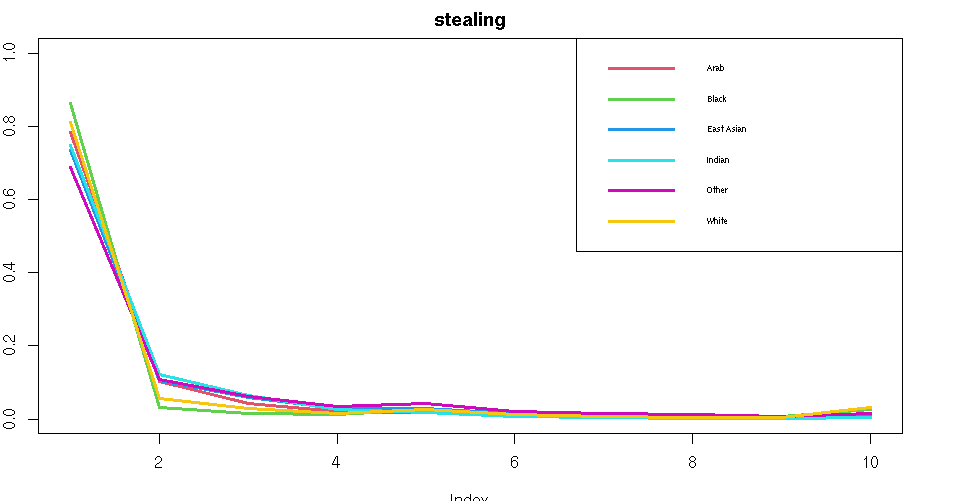
\includegraphics[scale=0.5]{ethsteal.jpeg}

Now let's look at the computed ethnicity effects.  These I calculate by ratio of sum of squares of difference from the mean curve of the particular ethnic curve and divide by sum of squares of the mean curve.  

% latex table generated in R 4.0.3 by xtable 1.8-4 package
% Mon May 10 01:22:03 2021
\begin{table}[ht]
\centering
\begin{tabular}{rlr}
  \hline
 & eth & explained \\ 
  \hline
1 & Arab & 0.09 \\ 
  2 & Black & 1.69 \\ 
  3 & East Asian & 0.34 \\ 
  4 & Indian & 0.41 \\ 
  5 & Other & 1.69 \\ 
  6 & White & 0.47 \\ 
   \hline
\end{tabular}
\end{table}

The inference we can draw from this is that on moral views about wrongness of stealing around the world, ethnic effects are miniscule.  

If you had any other opinions than this, if this is surprising to you, then what you need to do is understand that anti-stealing views originated millions of years ago in our ancestors in Africa, and were not adopted in the past few thousand years.  Therefore you can update your views and understand that at least for stealing the spectrum of views is universal.  To be clear, every ethnicity has a variety of views including 10=stealing is alway right at the right tail.  But the {\em distribution} is extremely invariant with negligible differences statistically.  

\section{Is This Trivia?}

Well maybe in half a century, it will be trivia, but today it certainly is not.  Racial prejudices regarding morality of people of different ethnicities is not only common but is a {\em plague} across the world that I intend to snuff out altogether.  These are measured high quality data from the World Values Survey.  

I recommend new prejudices that are not based on ethnicity but on other sorts of things.  

I am also 48 and have been around in many different situations.  I can tell you right now that people will be violently offended if you cast any doubts about their character.  Most likely they have self-control and will not pull out a pistol and shoot you right away, but they will definitely consider it.  Do not cast doubt about people's moral character.  It is dangerous in fact.  I am quite merciless against those who do it with me.

\end{document}